\title{Project 1}
\author{
        Jerry Duncan
}
\date{\today}

\documentclass[12pt]{article}

\usepackage{amsmath}
\usepackage{graphicx}
\usepackage{pythonhighlight}


\begin{document}
\maketitle

\section{Introduction}

Given a small, toy problem of trying to find a parking space to get ice cream, can we find the optimal policy that leads to us getting ice cream as soon as possible? First we must model the problem as a Markov Decision Process. Then, we can apply Value Iteration (and Policy Iteration) to iterate over the entire model and determine the expected amount of time it will take to get ice cream from each parking spot and whether or not it is occupied by a car. Then, after an apt amount of time, the values should converge and we can accurately use them to determine the best policy and what actions we should take to get ice cream as soon as possible.

\section{Markov Decision Process}

In order to model this problem as an MDP, we first need to determine what states there should be. For each parking space, we need to know if there is a car already in the parking space because it can mean the difference between crashing our car and getting no ice cream and parking and getting our ice cream really quickly. We also need to know what space we're at so we know how long it will take to walk to the ice cream shop if we park there. Because of this our state should be a tuple of (space number, free or taken). Once we have our states set, we just need to add transitions given each of the three actions we can take at a spot (wait, park, next). In Figure \ref{fig:mdp}, we can see what the entire problem modeled as an MDP would look like. Take note that at space M, where M is the last parking space, if we take the next action we no longer get ice cream and go to a terminal state.

\begin{figure*}
  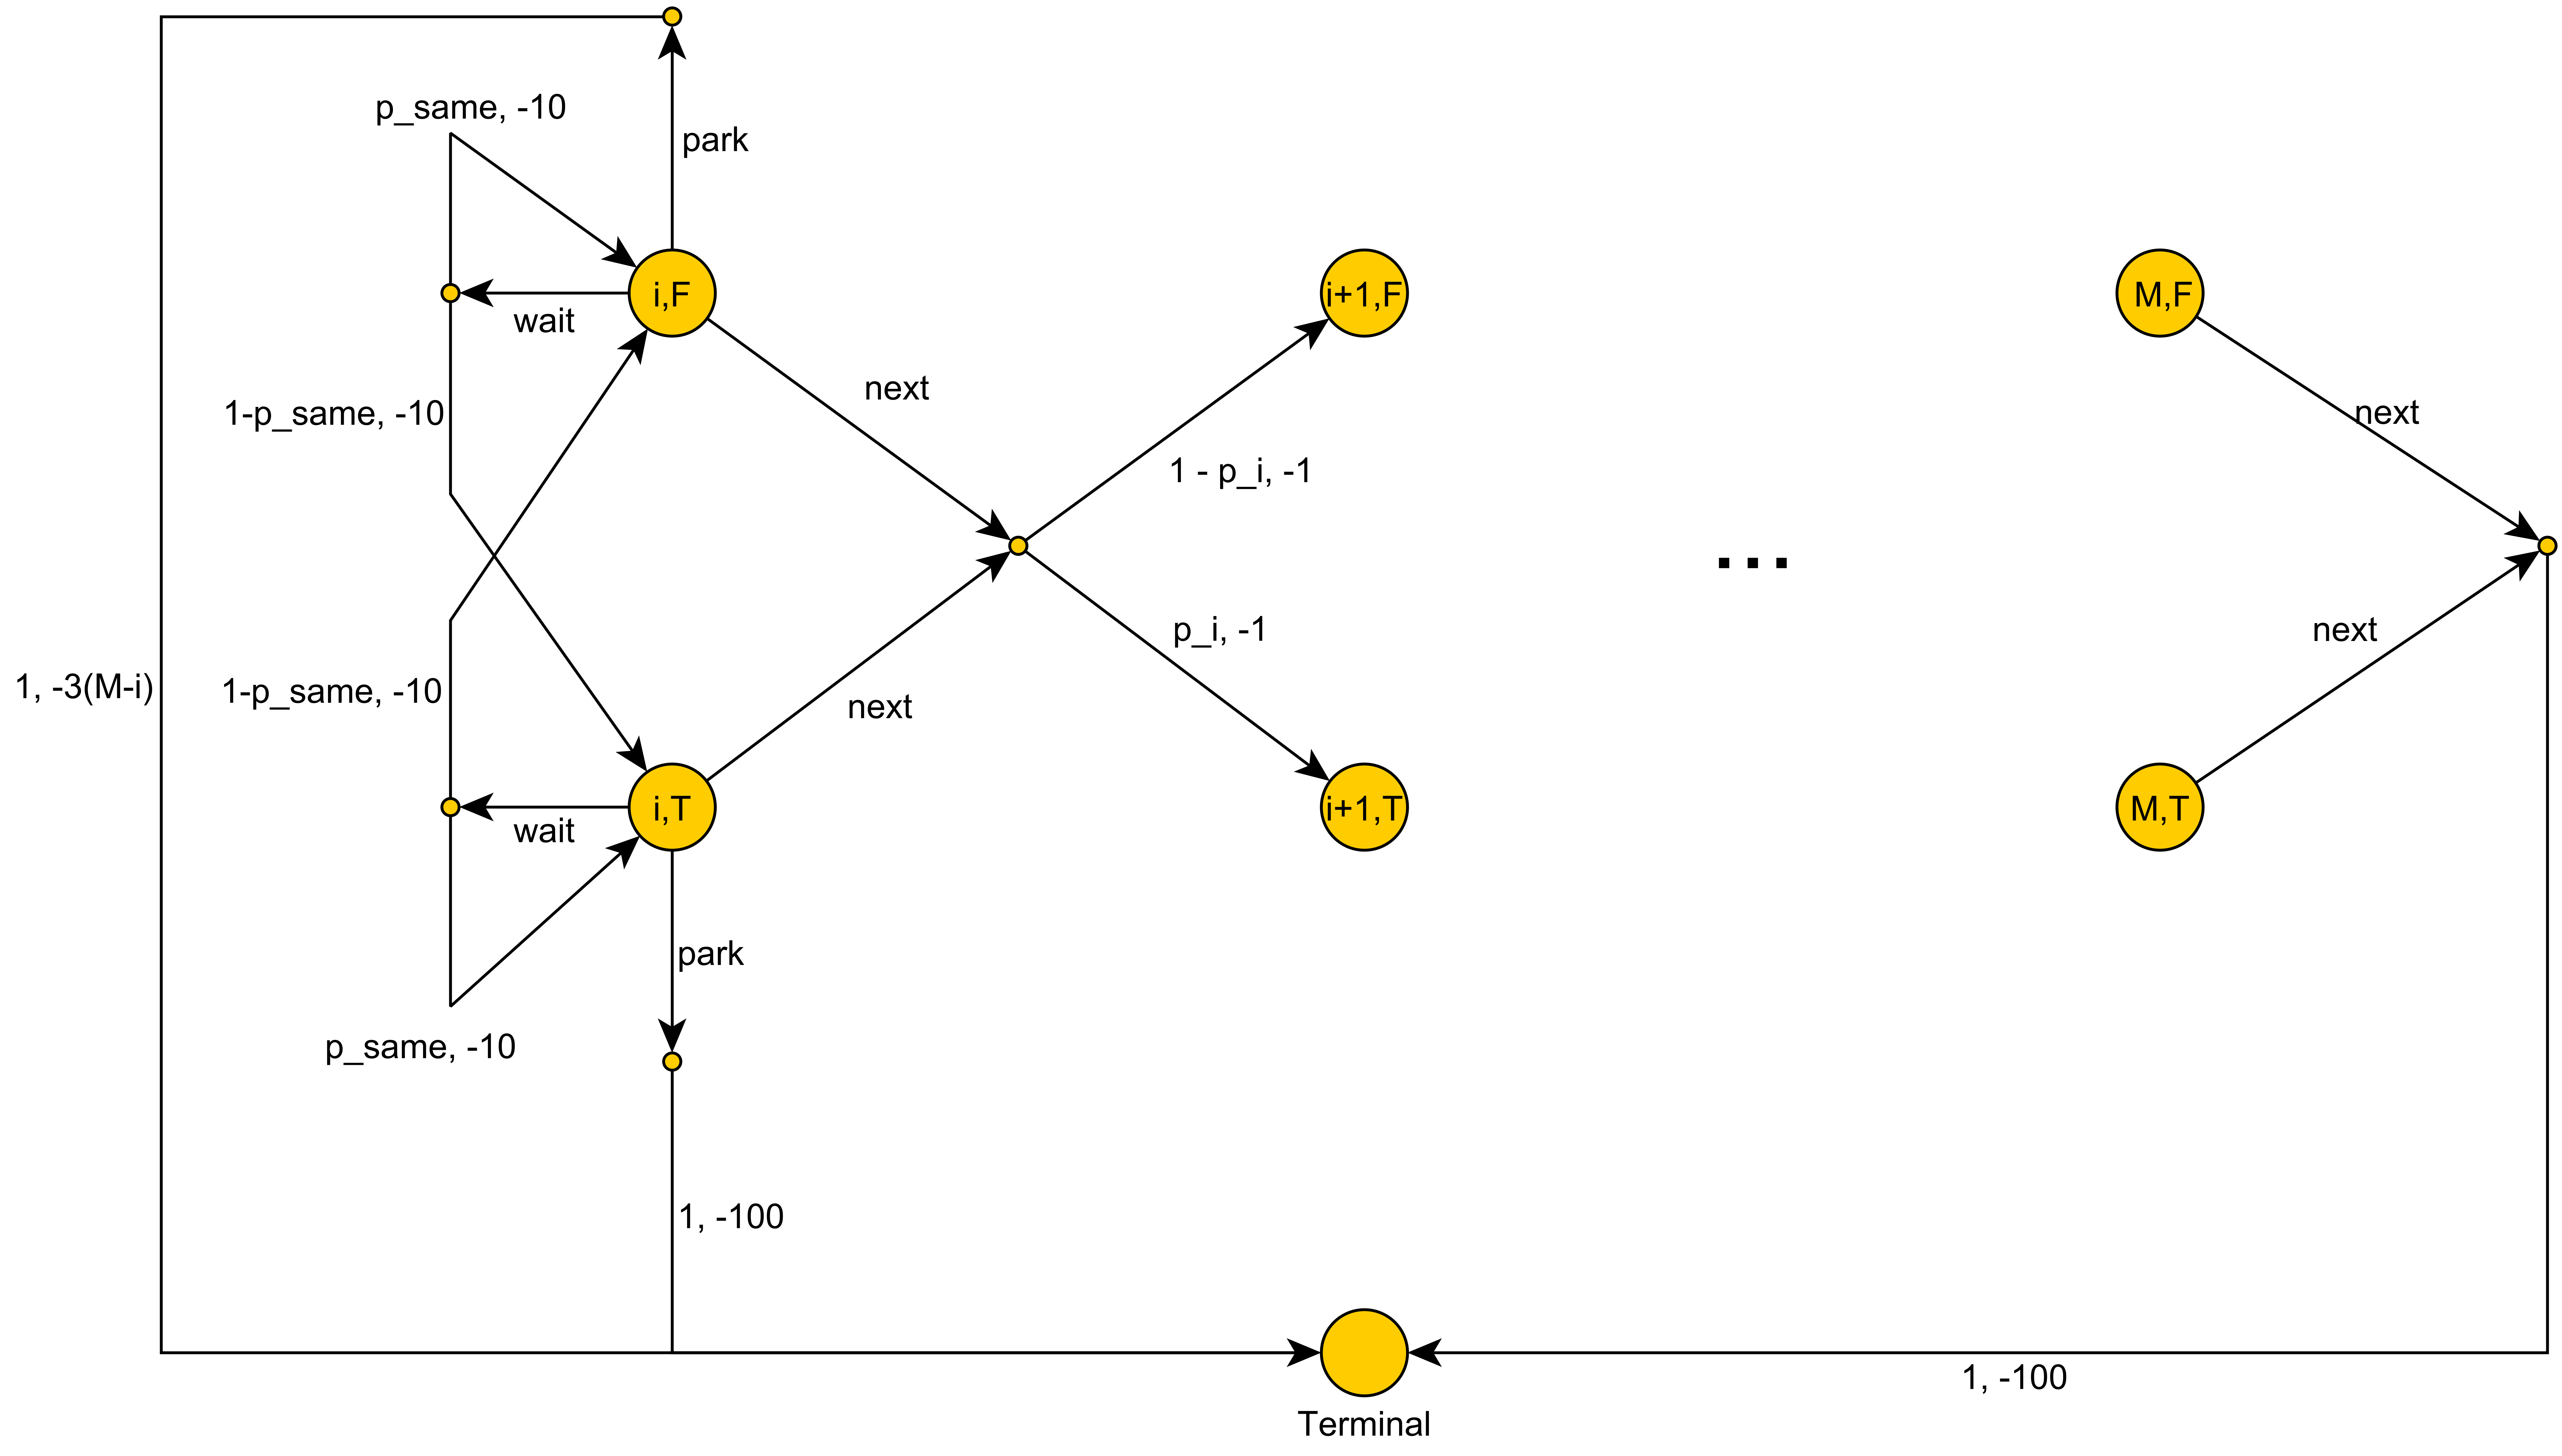
\includegraphics[width=0.95\linewidth]{Figures/MDP.png}
  \centering
  \label{fig:mdp}
  \caption{Ice Cream modeled as a Markov Decision Process}
\end{figure*}

\section{Code and Data Structures}

For V and Q, we need to store values for each space, state and in the case of Q, action. Since we have (M, 2) states and 3 actions, V is a 2d array with shape (M, 2) and Q is a 3d array with shape (M, 2, 3).

As for code, the reward function is a large set of cases for each action and space status pair. The value iteration function handles updating Q and V, one iteration at a time until a certain threshold is met or a maximum number of iterations occurs. The policy function just takes the max over the actions of Q (the last axis). Remember that while the policy finding part of value iteration could do a one-step ahead search over all the Q values again, since V has converged by the end of value iteration (and therefore the to-be selected Q values), we can use the argmax of the Q values as a valid replacement for recalculating the argmax over all of the actions again.

For the timing experiment in the Section \ref{sect:analysis}, times are gathered sequentially using \textit{time.time} and were not run multiple times. While that experiment is in no way extensive or extremely accurate as to individual runtime due to running each setting once, it can accurately show the increase in time over long runs.

\section{Results}

\paragraph{Part a}

In Table \ref{tab:value-fn}, we can see the final value function for this MDP, that is an estimate of the optimal value function. First let's look at the beginning of the parking lot. As we drive along, the probability of a space being open is very high for a long time, only decreasing by 0.8 / (M - 1) at each space we come to. Because driving to the next spot is so cheap (-1) compared to the extra -3 seconds we would incur from parking, the expected value of the first 4 spaces is less than just parking from those spaces. That's why the value function is the same in the empty and full 1-4 spaces. Once we get to space 5, the chance that a future space is open becomes increasingly less at every step, meaning that the value of a free space from space 5 and on is higher than continuing on and trying to get a further one (because the probability of the future spaces being open is slowly shrinking). Any other action's Q value is higher than just parking because of the small chance of the future spaces being open. When the space is full after space 4 and as the probability of future spaces being full increases greatly, the chance that we are either relinquished to getting no ice cream because all of the future spaces are full or having to wait at the final space and hope it opens up increases greatly. That's why the value function slowly increases for full spaces after 4 and eventually culminates to -100 for the last space because we run out of options and we would, on average, have to wait 10 times to get a space (-100), continue on and leave the parking lot (-100), or crash into a parked car (-100).

\begin{table}[]
  \centering
  \caption{Value function after convergence.}
  \label{tab:value-fn}
  \begin{tabular}{|c|c|c|}
    \hline
       & Empty  & Full    \\ \hline
    1  & -25.62 & -25.62  \\ \hline
    2  & -24.62 & -24.62  \\ \hline
    3  & -23.62 & -23.62  \\ \hline
    4  & -22.62 & -22.62  \\ \hline
    5  & -21    & -22.58  \\ \hline
    6  & -18    & -25.73  \\ \hline
    7  & -15    & -33.14  \\ \hline
    8  & -12    & -45.06  \\ \hline
    9  & -9     & -60.42  \\ \hline
    10 & -6     & -76.80  \\ \hline
    11 & -3     & -91.00  \\ \hline
    12 & 0      & -100.00 \\ \hline
  \end{tabular}
\end{table}

\paragraph{Part b}
The answer to this is very similar to part a. In Table \ref{tab:policy}, we can see the final policy of the MDP. So why does it make sense? Well, first let's look at empty spaces. As we get closer to the end of the parking lot, the best we can do is to park if it's empty. Waiting when it's free makes no sense anyway and the further along we keep going to the next space, the less likely the next space is actually open so we should take whatever we can get. Towards the beginning of the parking lot, however, is a different story. Because the chance of a parking space being empty past parking space 4 is still relatively high (60.9\%, 53.6\%, 46.4\%, ..., etc.), parking as soon as we can (space 1-4) isn't worth it and we should try to find a closer one.

Now let's look at the full spaces. In almost all cases, if a space is full, we should just go to the next one because if we were to park in it we would receive the worst reward (crashing). Similarly, waiting at each spot has the same probability of becoming empty, so if the reward is the highest for space M being empty, we might as well wait at that one.


\begin{table}[]
  \centering
  \caption{Policy after value function convergence}
  \label{tab:policy}
  \begin{tabular}{|c|c|c|}
    \hline
       & Empty & Full \\ \hline
    1  & next  & next \\ \hline
    2  & next  & next \\ \hline
    3  & next  & next \\ \hline
    4  & next  & next \\ \hline
    5  & park  & next \\ \hline
    6  & park  & next \\ \hline
    7  & park  & next \\ \hline
    8  & park  & next \\ \hline
    9  & park  & next \\ \hline
    10 & park  & next \\ \hline
    11 & park  & next \\ \hline
    12 & park  & wait \\ \hline
  \end{tabular}
\end{table}

\section{Analysis} \label{sect:analysis}

\paragraph{Question 1} One of the most important things when picking a Reinforcement Learning algorithm to solve a real-world problem is not only how well it solves the problem but how quickly can it solve the problem. Those reasons are part of the inspiration behind using Monte Carlo methods and Temporal Difference learning. So, if we scale this problem to take on more parking spaces, how well does the time it take to solve it scale?

For this question I've setup an experiment to run the value iteration function from 10 to 1,000 spaces in increments of 5. Because the larger amount of spaces take a large amount of time, I didn't run each number of steps more than once so some of the times are potentially inaccurate due to CPU scheduling and other factors, but it can still accurately show the increase in time across the 198 different experiments. In Figure \ref{fig:time-vs-spaces}, we can see the a plot of the time taken versus the number of states. We can see from this plot that the time is increasing as a linear function of the number of spaces. We can further verify this in Figure \ref{fig:time-per-space}, to see that the time taken per space starts to converge to $0.0055$ seconds. To further see this and to see where it lies compared to other linear functions, I've plotted $0.01x$, $0.0055x$, and $0.001x$ in Figure \ref{fig:time-vs-estimates}. From this figure we can firmly see that the runtime of this problem behaves a lot like $0.0055x$.
When we do later projects using other methods of solving value functions, we can go perform experiments to compare their asymptotic runtime to Dynamic Programming's.

\paragraph{Verification} So the last thing we want to ask ourselves about these graphs is does this behavior make sense?
Let's first take a look at how we expect it to behave for the base case of 12 spaces. We have a bounded while loop that runs until convergence or 1,000 iterations occur. We then iterate over each of \textit{N} states and \textit{M} actions, and \textit{at most} perform calculate two values. For this base case we would then expect the strict upper bound to be $1,000 * M * N * 2 = 1,000 * 12 * 3 * 2 = 72,000$ calculations (not including additions or lookups which there are a minimal amount). And as we extend this problem to larger parking lots, the only number that should change is \textit{M}, because regardless of parking lot size, there are a set number of actions and still, at most, two calculations needed for each Q value. We should then expect that it behaves like O($1,000 * 3 * 2 * M$) = O(\textit{M}). In other words, it does make sense that this problem behaves linearly as a function of \textit{M}

\paragraph{Side note} These timing experiments are in no way comprehensive and also don't deal with the fact that the rewards don't scale the same as states. Regardless, it is still an interesting observation that should be able to be directly compared with future value function solvers.

\begin{figure*}
  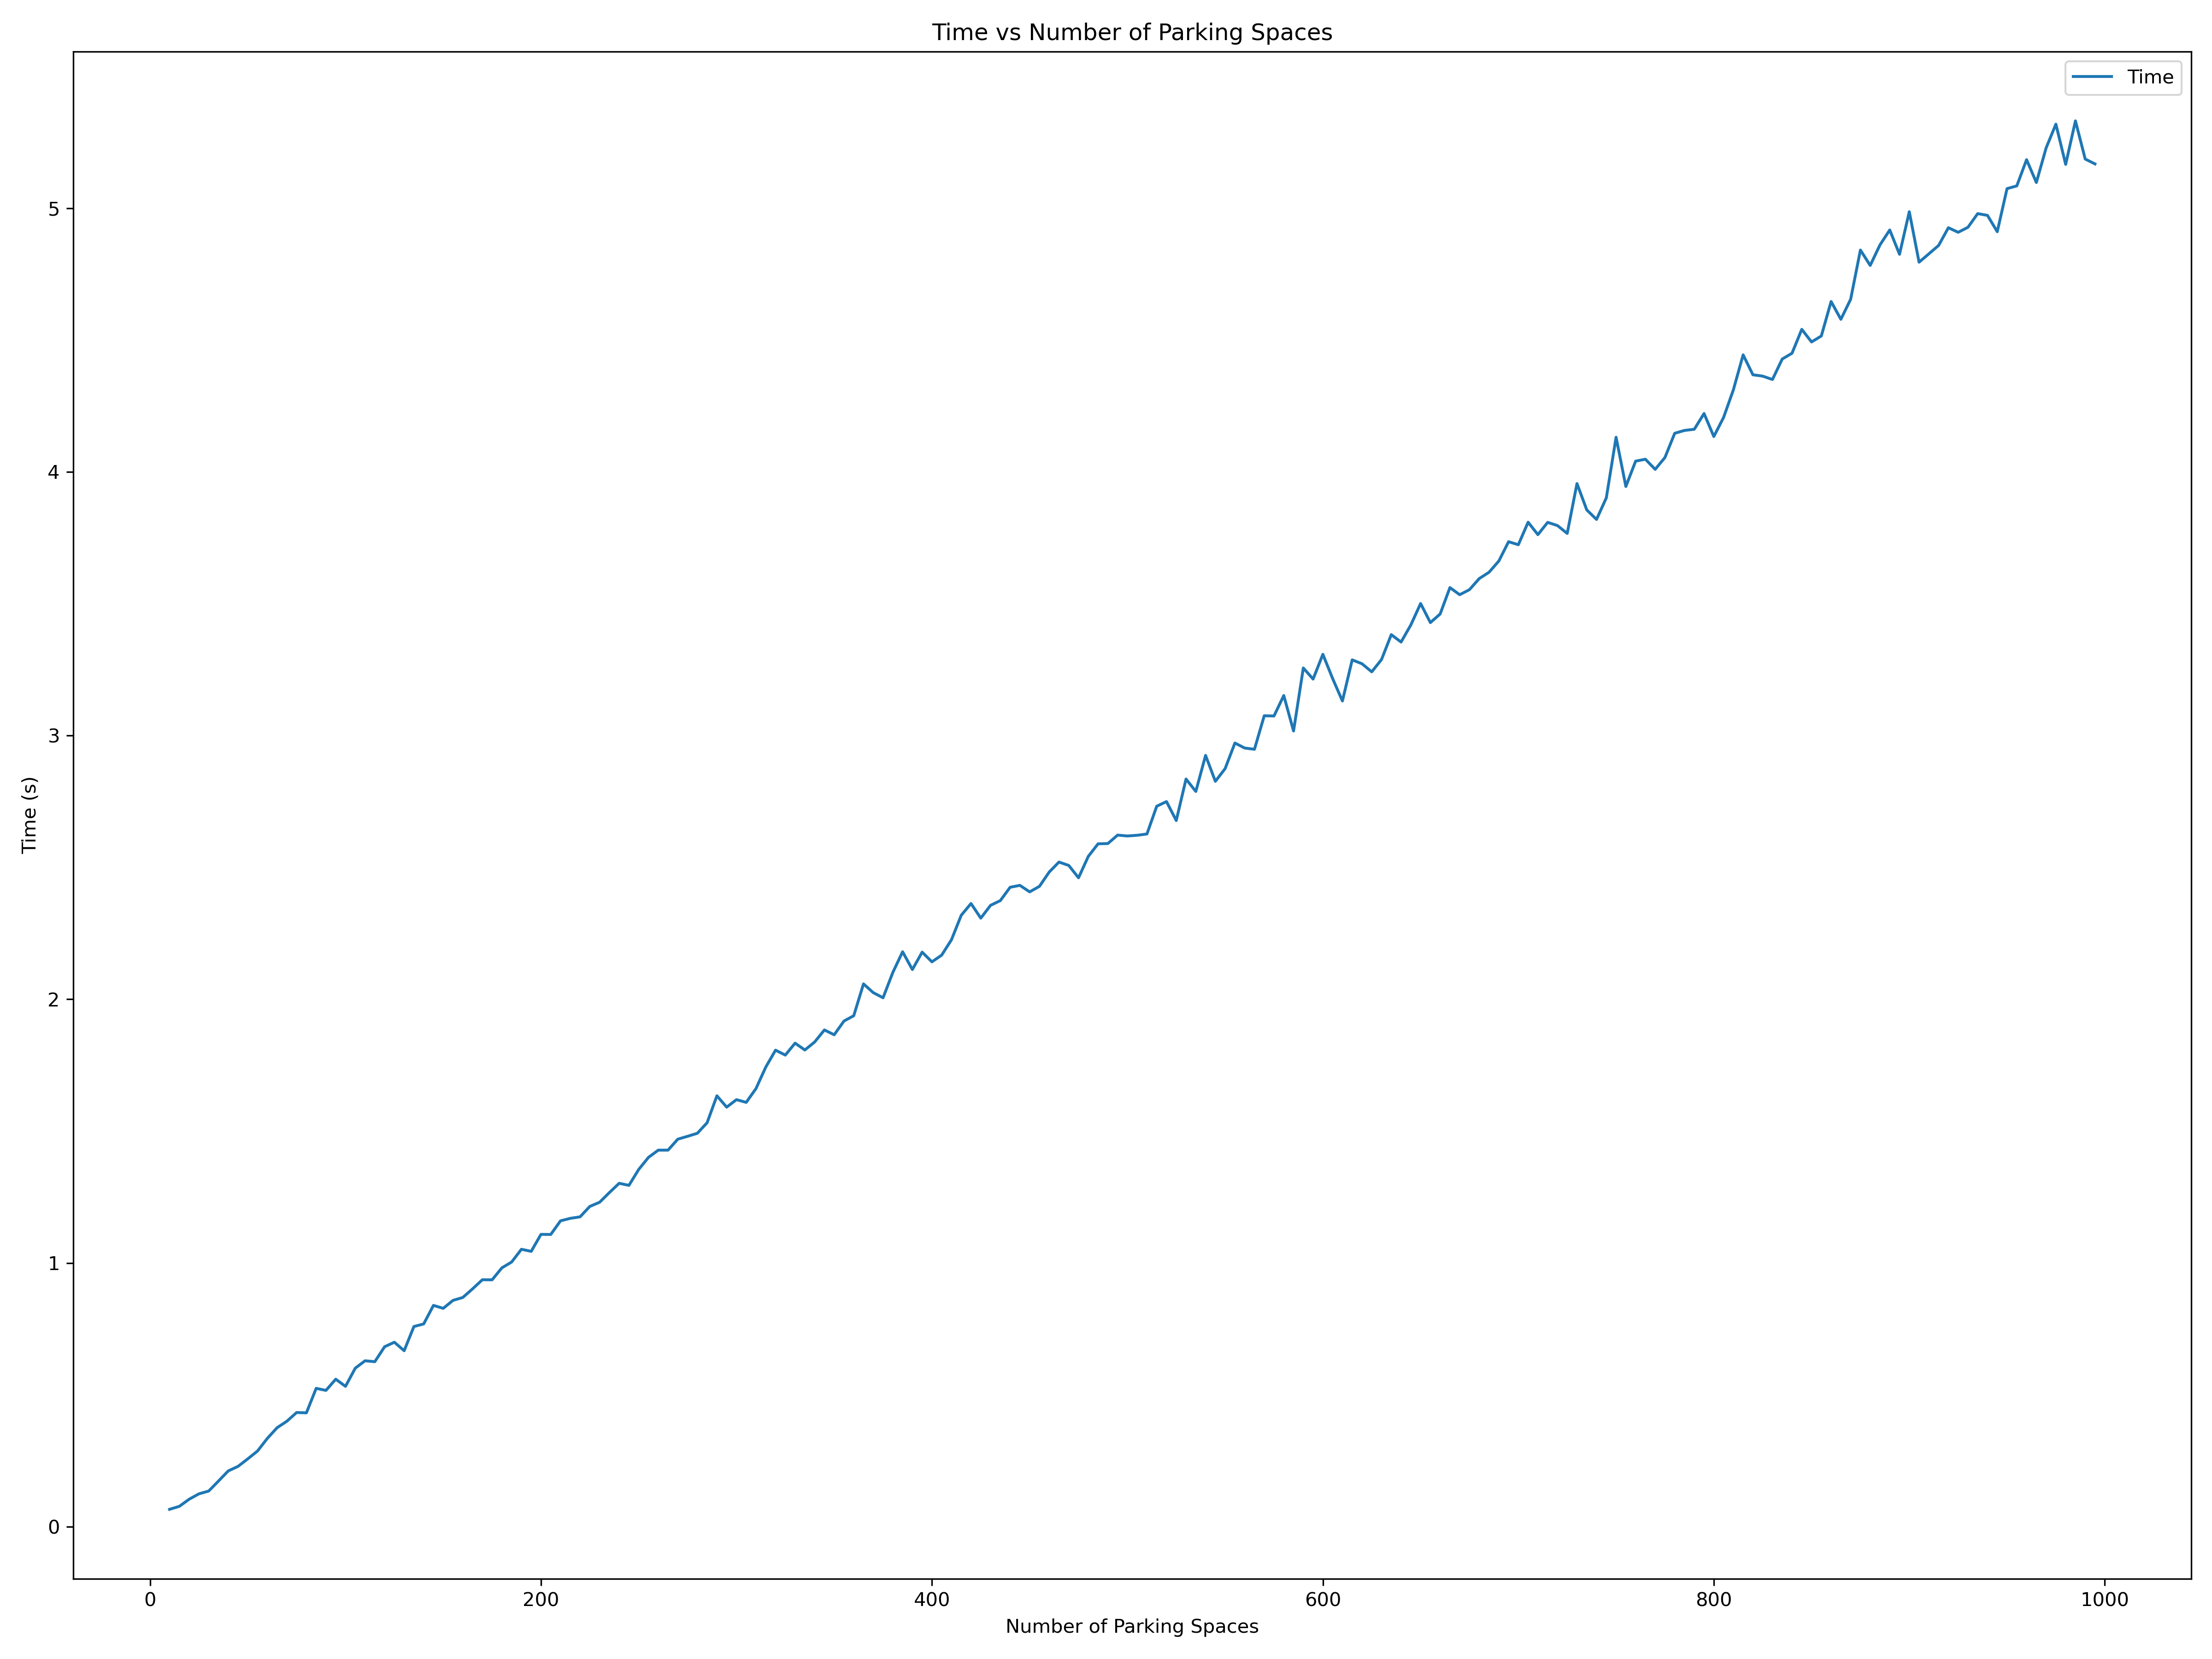
\includegraphics[width=0.95\linewidth]{Figures/time_vs_spaces.png}
  \centering
  \label{fig:time-vs-spaces}
  \caption{Time vs number of spaces}
\end{figure*}

\begin{figure*}
  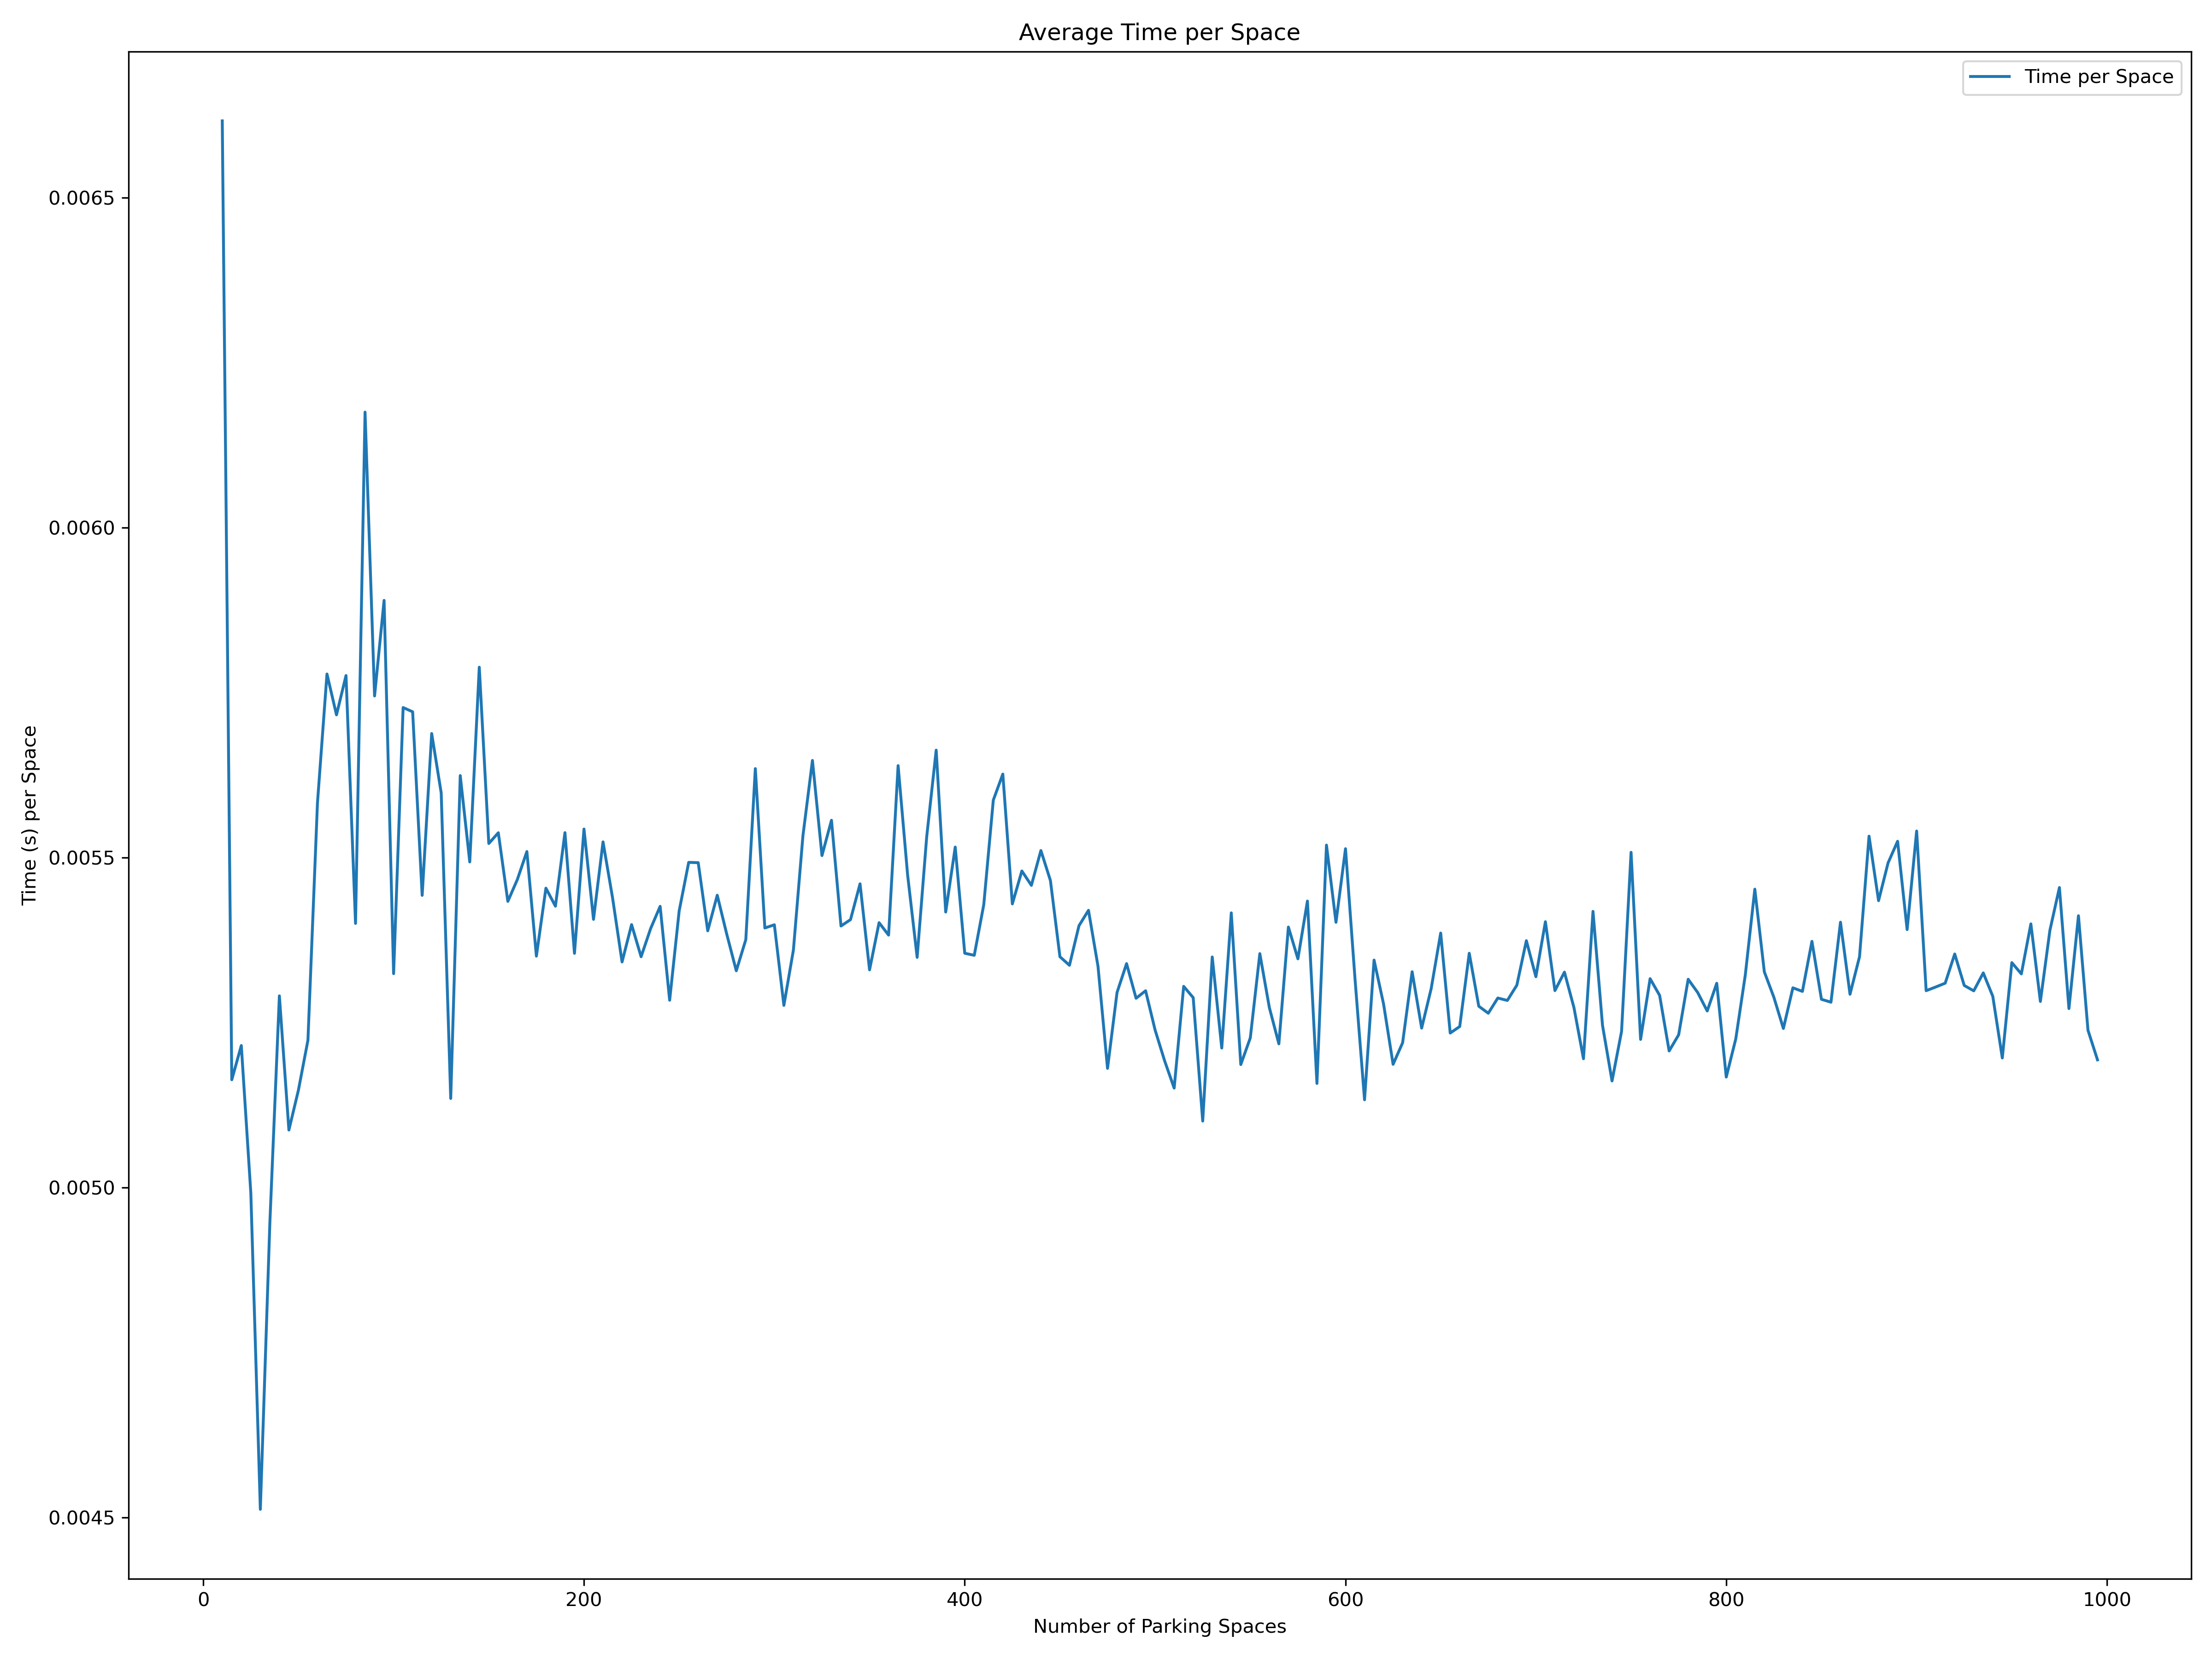
\includegraphics[width=0.95\linewidth]{Figures/time_per_space.png}
  \centering
  \label{fig:time-per-space}
  \caption{Time taken per space}
\end{figure*}

\begin{figure*}
  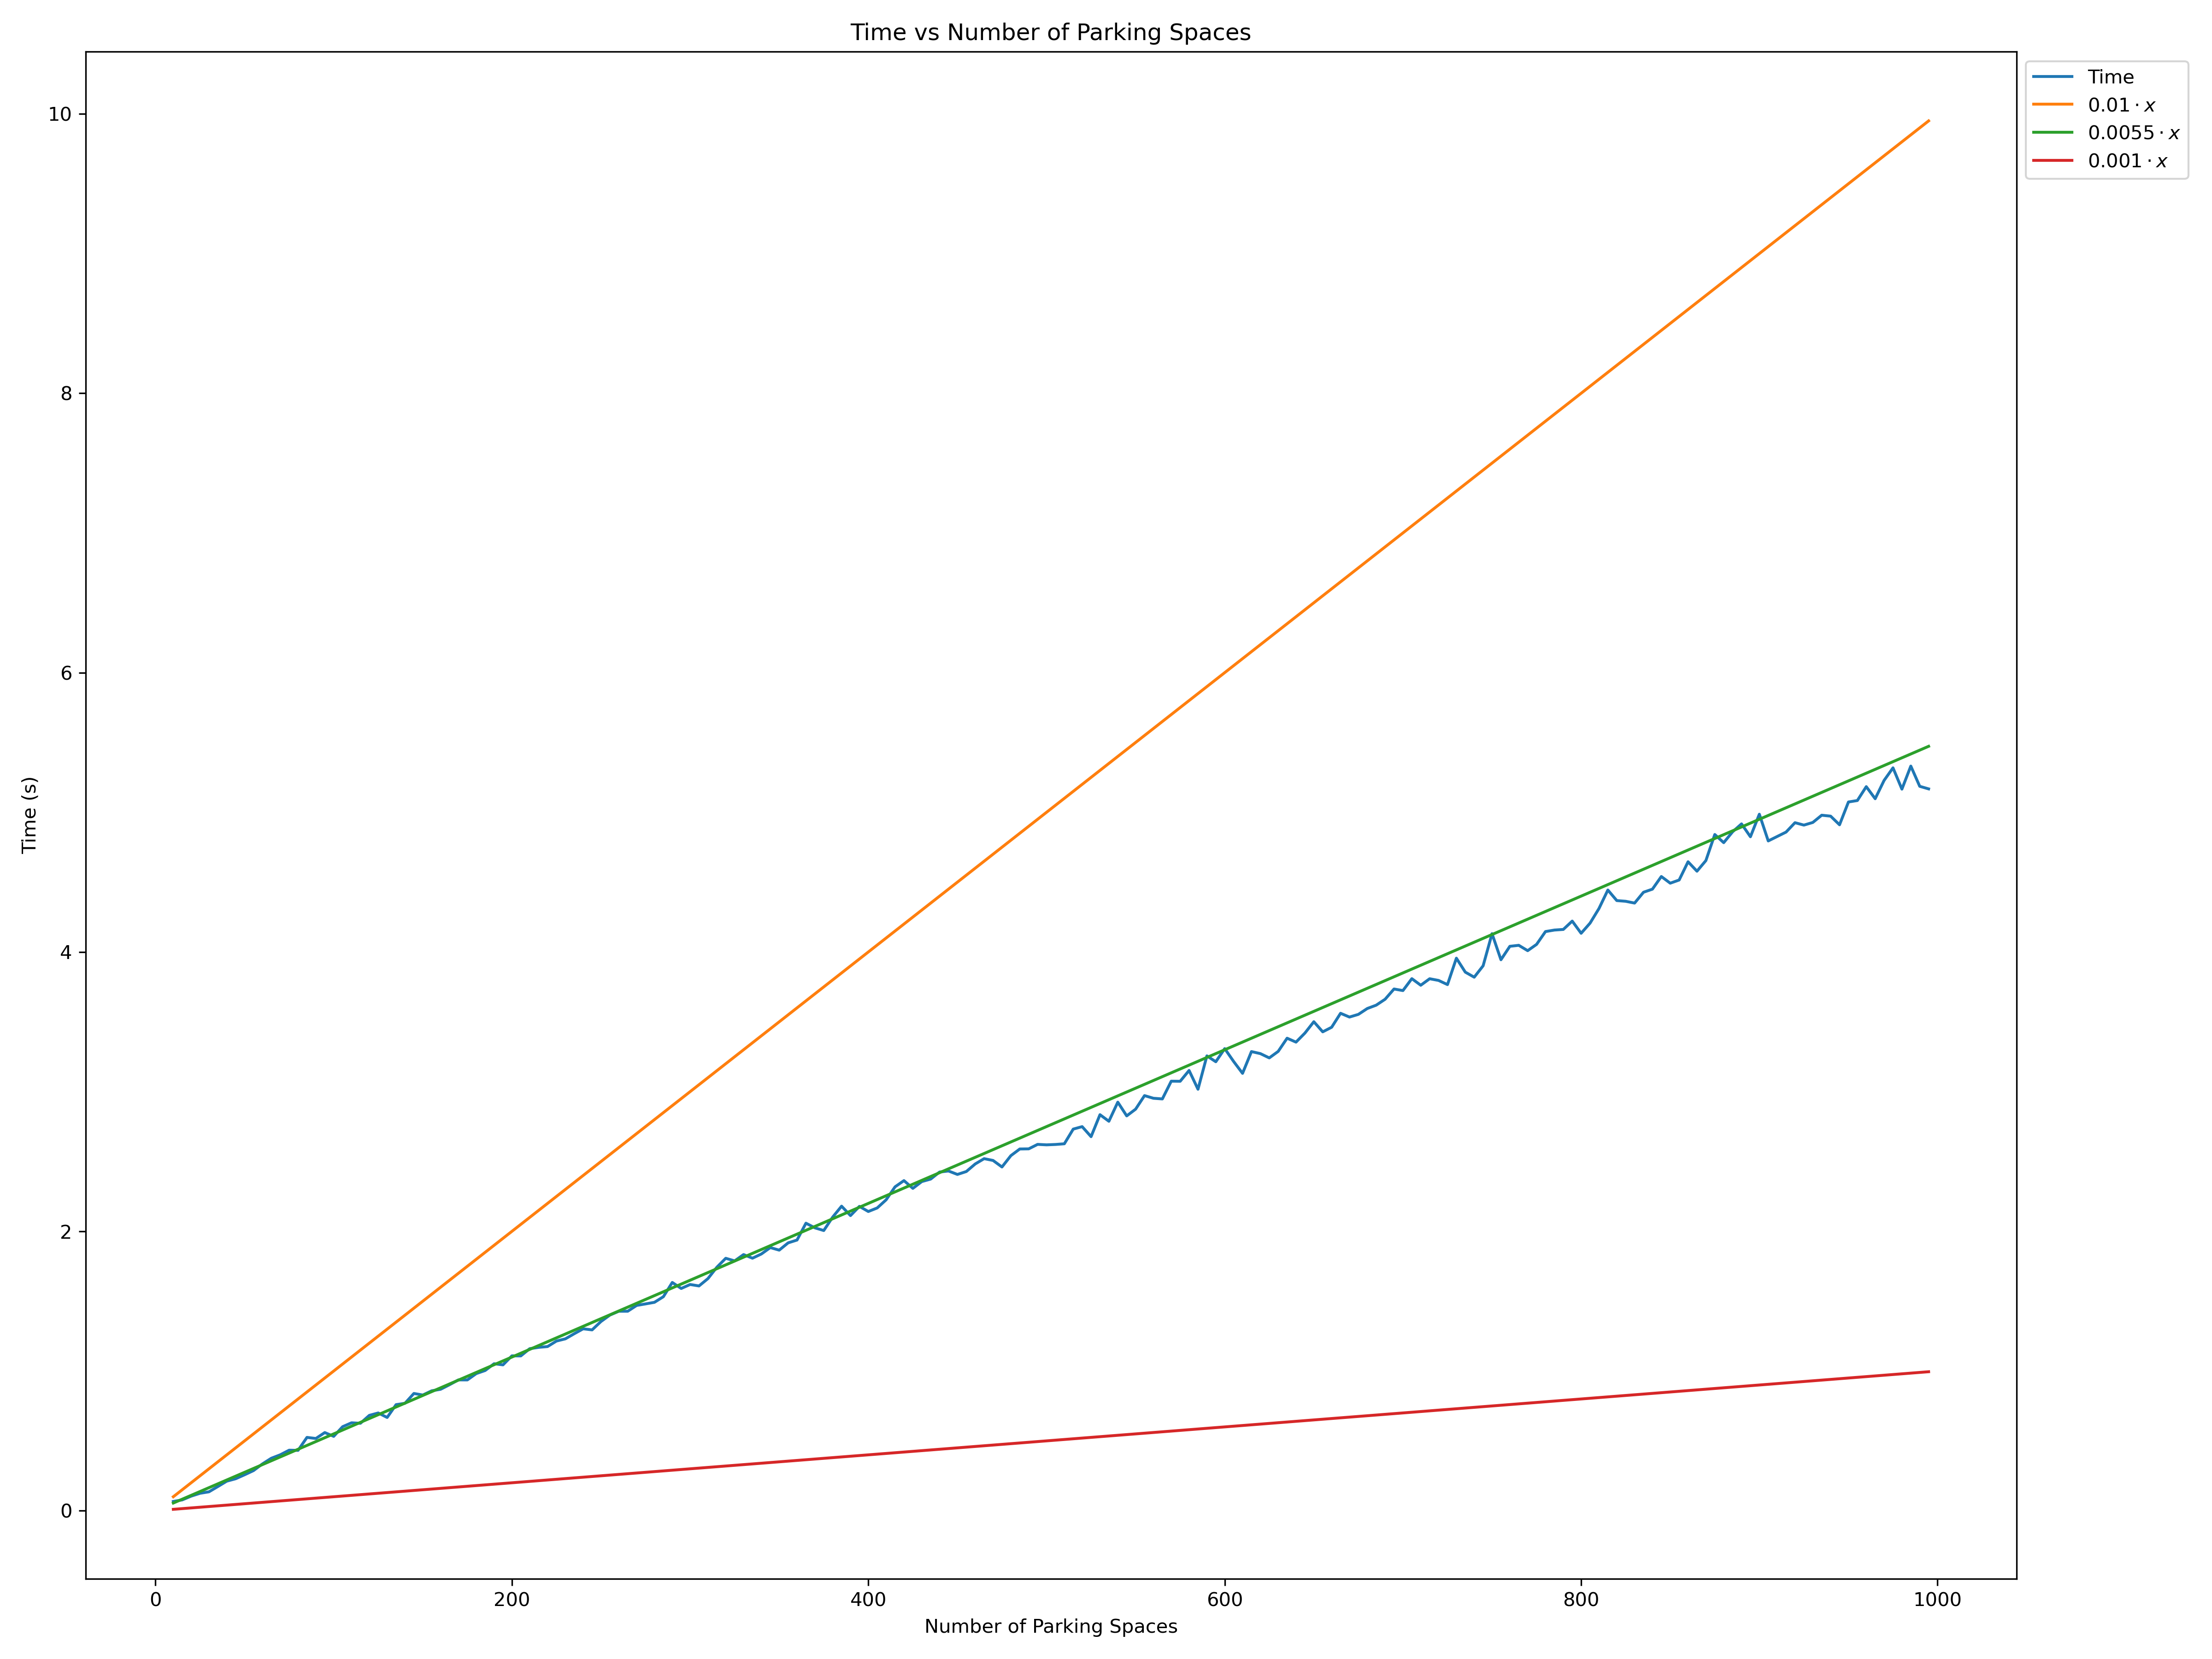
\includegraphics[width=0.95\linewidth]{Figures/time_vs_spaces_with_estimates.png}
  \centering
  \label{fig:time-vs-estimates}
  \caption{Time vs number of spaces with function estimates}
\end{figure*}

\paragraph{Question 2} Next, I wanted to compare value iteration and policy iteration. Through all of my testing, both converge to the same final optimal policy. While this is expected, it is a good indicator that I am performing policy iteration correctly. So how can we compare the two? The most direct way is to look at how many iterations value iteration goes through and how many policy iteration goes through across however many cycles. For my value iteration function, it iterates over all the complete state and action spaces $154$ times. This is with a $V$ and $Q$ initialization of all 0's. As for policy iteration, it depends a lot on the initial policy as some policies are harder to converge than others. In Figure \ref{fig:policy-iteration-1} and Figure \ref{fig:policy-iteration-2} I show a couple examples of how the policies evolve over time as well as the number of iterations policy evaluation went through. As we can see from these figures, sometimes the initial policy causes policy evaluation to hit the cap of $1,000$ iterations without converging. Figure \ref{fig:policy-iteration-1} is one of the better runs I was able to generate so even in one of its better cases, policy iteration took $193 + 9 + 12 + 2 = 216$ iterations, which is worse than value iteration's $154$. It would seem likely that for this problem, value iteration is vastly better than policy iteration in most cases and on the off chance the initial policy of policy iteration is decent, it still seems to be marginally better.

\begin{figure*}
  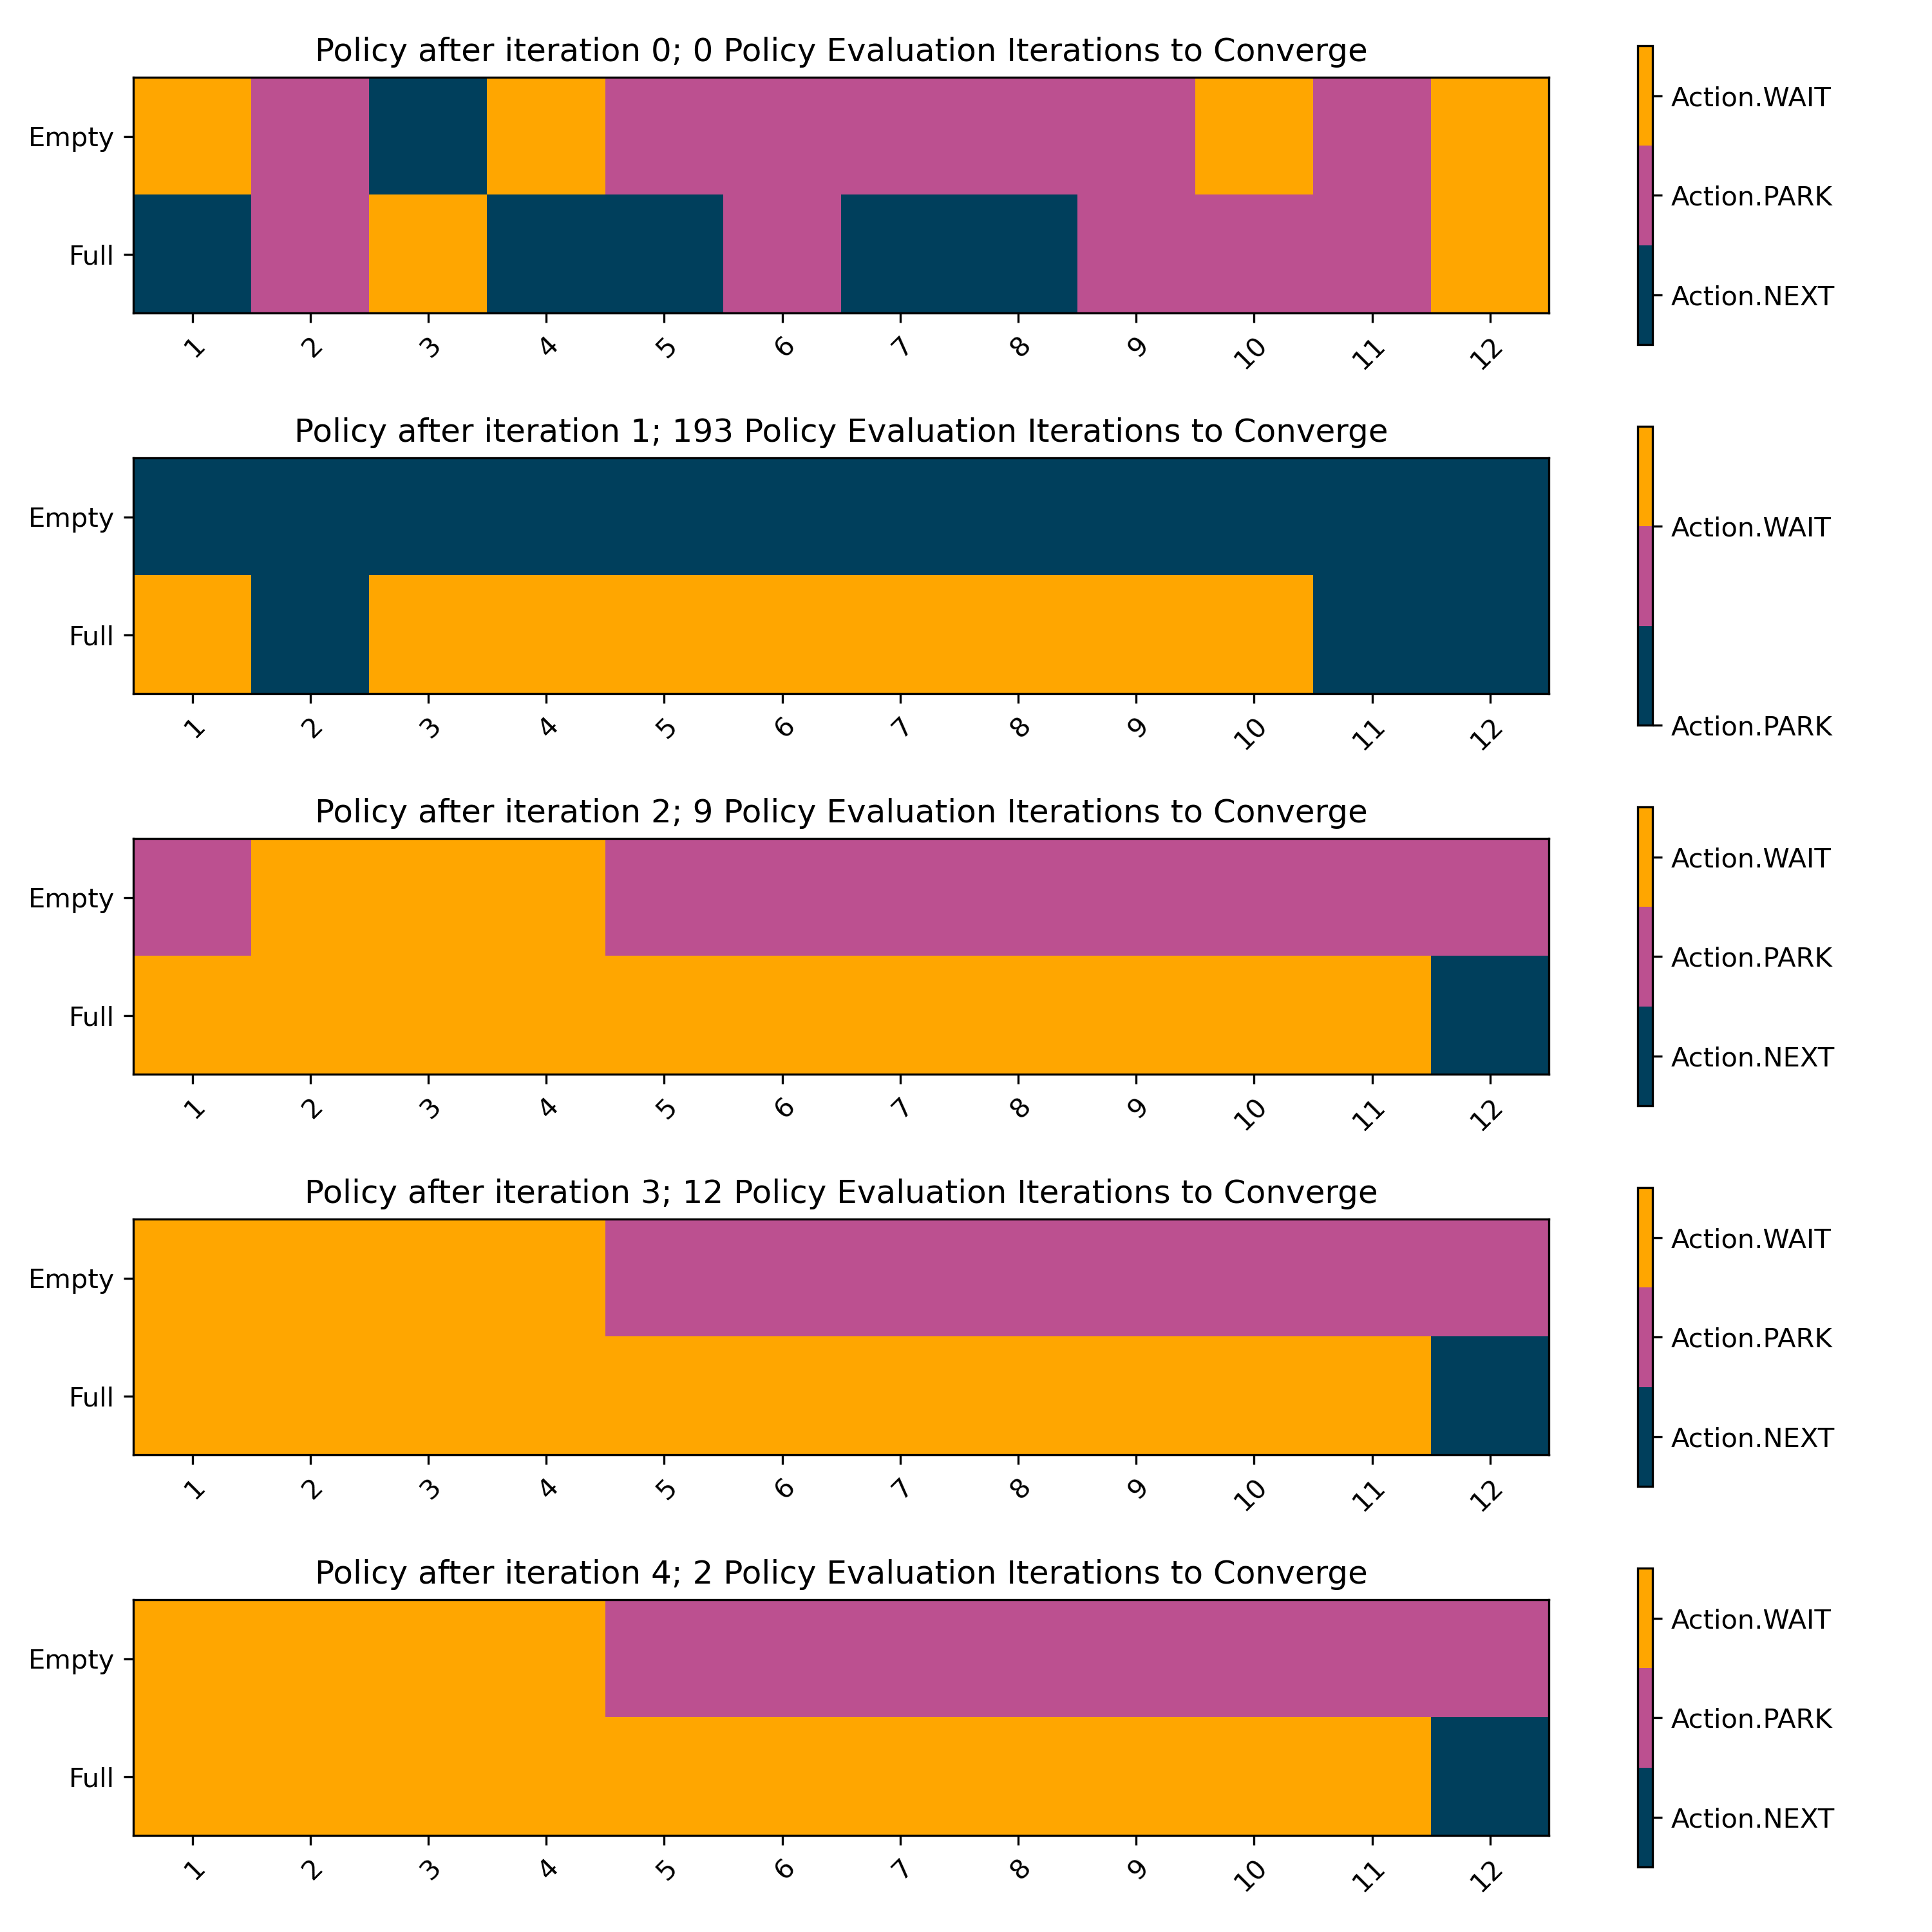
\includegraphics[width=0.95\linewidth]{Figures/policy_iteration_policies_1.png}
  \centering
  \label{fig:policy-iteration-1}
  \caption{Policy Iteration With Random Initialization 1}
\end{figure*}

\begin{figure*}
  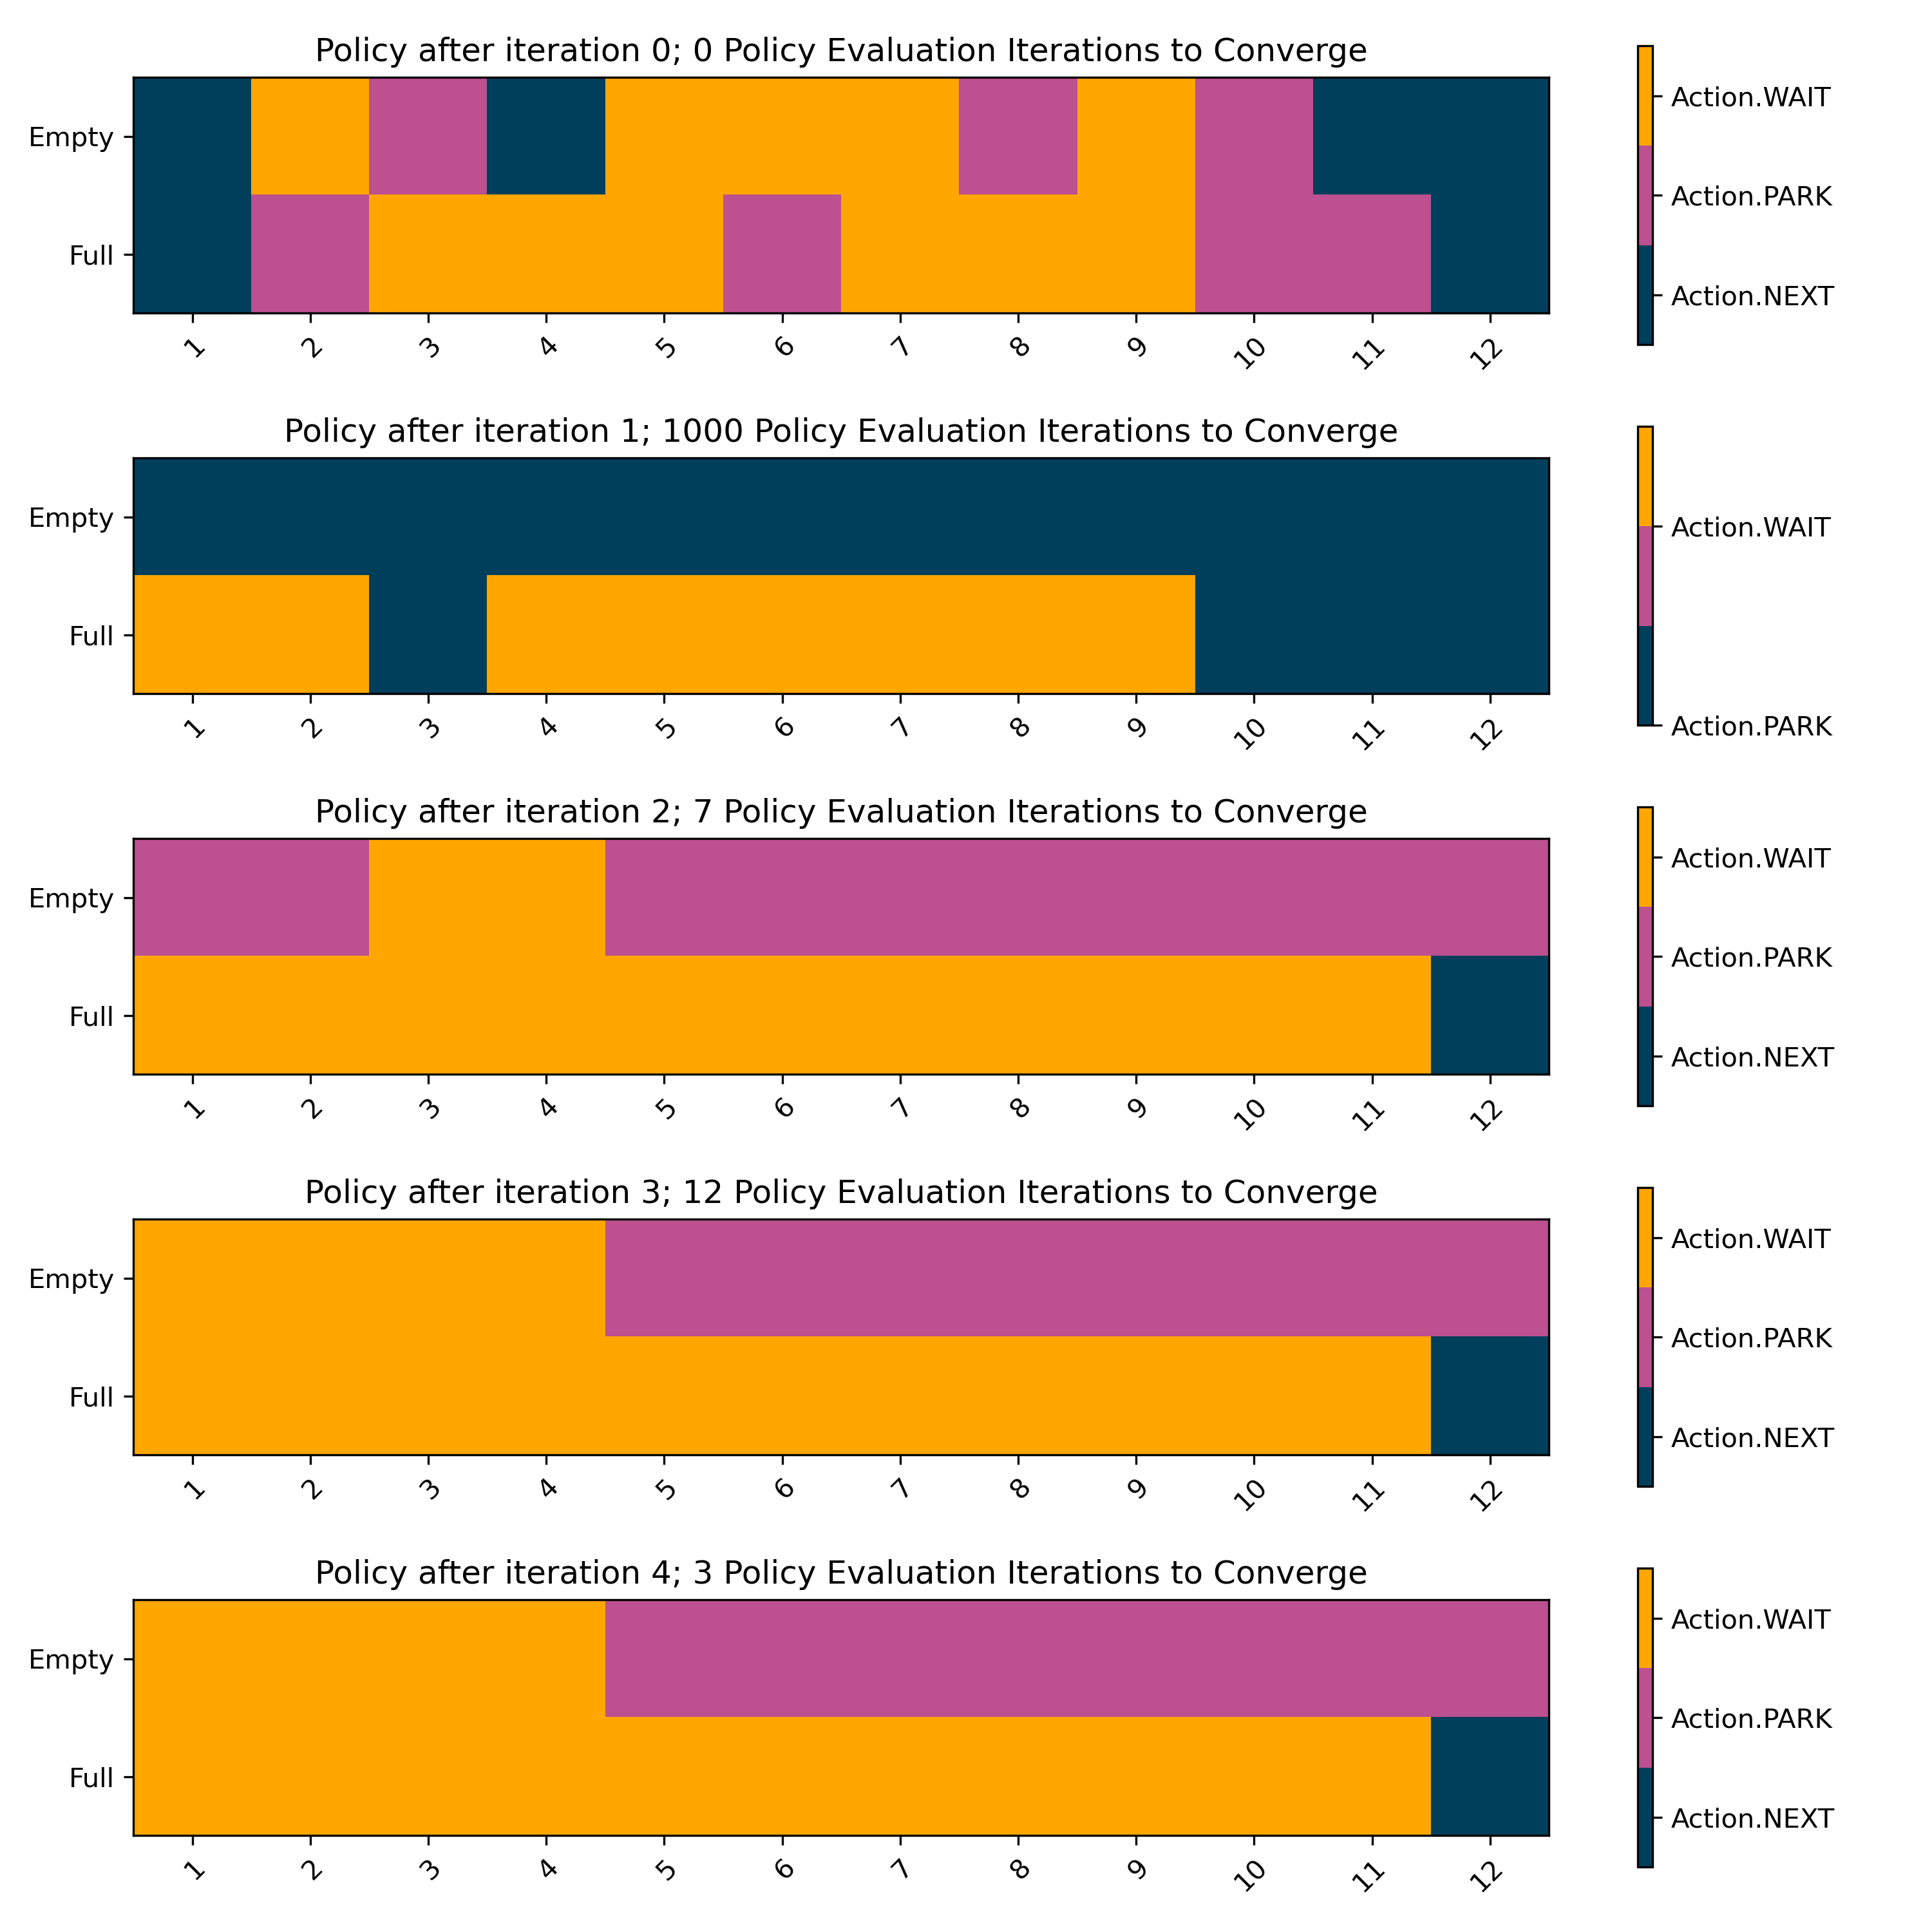
\includegraphics[width=0.95\linewidth]{Figures/policy_iteration_policies_2.png}
  \centering
  \label{fig:policy-iteration-2}
  \caption{Policy Iteration With Random Initialization 2}
\end{figure*}

\section{Conclusion}

Overall, in this project I've achieved creating a solution to the problem by forming it as an MDP and applying both value and policy iteration to compare their differences. I've also tested the time it takes for value iteration to work across a large number of states and determined that while DP is pretty fast, especially since it's linear, it can still be relatively slow.

I've learned that dynamic programming methods are pretty powerful in solving reinforcement learning problems that can be formed as MDPs. And that while policy iteration does work, it's not nearly as fast as value iteration.

\bibliographystyle{abbrv}
\bibliography{main}

\end{document}